\documentclass[10pt,paper=a4,final]{scrartcl}
\usepackage[utf8]{inputenc}
\usepackage{tabularx}		%used for the tables
\usepackage{geometry}		%allows us to specify the 'seitenrand'
\usepackage[table]{xcolor}	%allows us to make colored fields in the tables
\usepackage{graphicx}		%package used to include graphics
\usepackage{hyperref}   	%used to make klickable links

%\hypersetup{linktocpage}	%make the tableofcontent klickable
\hypersetup{
  colorlinks,
  citecolor=black,
  filecolor=black,
  linkcolor=black,
  urlcolor=black
}

\setcounter{tocdepth}{4}	%include paragraph in tableofcontents
\setcounter{secnumdepth}{5}	%also number the paragraphs

%These two lines will allow us to specify our own headers/footers
\usepackage{fancyhdr}
\pagestyle{fancy}
 \setlength{\parskip}{0pt}
 \setlength{\baselineskip}{0pt}

%The next three lines set the default font to Arial
%use 'getnonfreefonts arial-urw' to install uarial on Linux systems
\usepackage[T1]{fontenc}
\usepackage[scaled]{uarial}
\renewcommand*\familydefault{\sfdefault}

\geometry{a4paper, top=20mm, right=20mm, bottom=20mm, left=20mm}
\title{Voranalysebericht}
\author{Bash Vi, Shylux, Kaleb Tschabolt}
\date{\today}

%defining header and footer
\fancyhf{}	%delete default values
\setlength{\headwidth}{\textwidth}	%header and footer width equal the text width
\fancyhead[LE,LO]{
\includegraphics[scale=0.6]{header.png}}
\fancyhead[RE,RO]{ProjectExplorer}
\fancyfoot[CE,CO]{Speicherdatum: \today{}}
\fancyfoot[RE,RO]{\thepage}

\begin{document}
\maketitle
\newpage
\begin{tabularx}{\textwidth}{ r X }	%X fields are stretched over the whole space
\textcolor{white}{{\bf Status}}\cellcolor{blue!80!} & {\bf In Arbeit}/In Prüfung/Abgeschlossen\cellcolor{blue!20!} \\
\textcolor{white}{{\bf Projektname}}\cellcolor{blue!80!} & Projektexplorer\cellcolor{blue!20!} \\
\textcolor{white}{{\bf Projektleiter}}\cellcolor{blue!80!} & Niklaus Hofer\cellcolor{blue!20!} \\
\textcolor{white}{{\bf Auftraggeber}}\cellcolor{blue!80!} & M. Frieden, GIBB\cellcolor{blue!20!} \\
\textcolor{white}{{\bf Autoren}}\cellcolor{blue!80!} & Niklaus Hofer\cellcolor{blue!20!} \\
\textcolor{white}{{\bf Verteiler}}\cellcolor{blue!80!} & Lukas Knöpfel, Kaleb Tschabolt, Niklaus Hofer\cellcolor{blue!20!}
\end{tabularx}
\newline
\newline
\newline
{\bf Änderungskontrolle, Prüfung, Genehmigung}
\newline

\begin{tabularx}{\textwidth}{l l X X}
\textcolor{white}{Version}\cellcolor{blue!80!} & \textcolor{white}{Datum}\cellcolor{blue!80!} & \textcolor{white}{Beschreibung, Bemerkung}\cellcolor{blue!80!} & \textcolor{white}{Name oder Rolle}\cellcolor{blue!80!} \\
\cellcolor{blue!20!} 1& \cellcolor{blue!20!} \today{} & \cellcolor{blue!20!} & Niklaus Hofer, Projektleiter\cellcolor{blue!20!} \\
\end{tabularx}
\newline
\newline
\newline
{\bf Definitionen und Abkürzungen}
\newline

\begin{tabularx}{\textwidth}{l X}
\textcolor{white}{Begriff/ Abkürzung}\cellcolor{blue!80!} & \textcolor{white}{Bedeutung}\cellcolor{blue!80!} \\
\cellcolor{blue!20!} & \cellcolor{blue!20!} \\
\end{tabularx}
\newline
\newline
\newline
\bibliographystyle{plain}
\bibliography{voranalyse}{}
\flushleft
\newpage
\tableofcontents
\newpage

\section{Zweck des Dokuments}
In der Voranalyse geben wir einen groben Einblick in die künftigen Funkionen unseres Programmes. Hier werden die Ziele festgesetzt und Entscheidungen \"uber die zu verwendeten Technologien begründet und festgehalten.
\section{Ist-Aufnahme und Ist-Analyse}
\subsection{Beschreibung des Ist-Zustands (Ist-Analyse)}
\begin{itemize}
  \item Da das Projekt neu gestartet wird, existiert keine Vorarbeit, auf der wir aufbauen könnten.
  \item Einige der Ideen können aber mit denjenigen von Gnome Zeitgeist\cite{activity_journal} und Apple timemachine\cite{timemachine} verglichen werden.
  \item Als bestehende Lösung könnte man die herkömmliche, hierarchische Struktur von Dateisystemen ansehen. Allerdings wollen wir diese nicht ersetzen, sondern lediglich um weitere Möglichkeiten ergänzen.
\end{itemize}
\subsection{Schwachstellenanalyse}
\begin{itemize}
  \item Es existiert zwar kein Vorsystem, dessen Schwächen wir hier beschreiben könnten. Ich möchte hier aber auf die Schwächen herkömmlicher Dateiverwaltungssysteme eingehen.
  \item Diese haben vorallem das Problem, dass sich die Anwender herkömmlicher Dateisysteme eine Dateistruktur ausdenken und merken müssen. Sollten sie die Struktur jemals vergessen, so ist es schwierig Dateien zu finden. Auch ist das System recht unflexibel, wenn es darum geht Dateien, die zum gleiche Thema gehören, die aber weit über die hierarchische Struktur verteilt sind, zusammen zu verwalten.
\end{itemize}
\subsection{Sicherheit}
Es existieren keine Vorsysteme, die daher auch keine Sicherheitsl\"ucken aufweisen k\"onnen. \\
Erw\"ahnenswert scheint hier aber, einmal mehr, das cloud computing. Alle Daten bei einem storage Anbieter zu lagern löst nicht nur das Problem der Backups, sondern erlaubt auch das blitzschnelle Durchsuchen der Dokumente, da viele der online Anbieter (insbesondere Google mit seinem online Office) die Dokumente indexieren und so das Durchsuchen mit komplexen Algorithmen erlauben. All diese Vorteile haben aber einen entscheidenden Nachteil: Die Kontroller \"uber die Dateien geht verloren. Der Storage-Anbiter hat, sofern man die Daten nicht manuell verschl\"usselt, vollen Zugriff darauf. Zudem besteht hier der Nachteil dass ein Angreiffer alle die Daten bequem einsehen wenn er an das Passwort kommt.
\subsection{Zuk\"unftige Entwicklung}
Das Gnome Zeitgeist Projekt\cite{activity_journal} setzt einige innovative Ideen um, die das verwalten von Dateien komfortabler machen sollen.
Dabei geht es darum, dass dokumentiert wird wann welche Dateien geöffnet wurden und welche anderen zur selben Zeit geöffnet waren. Es ermöglicht dann nicht nur die chronologische Ansicht der Dateien, sondern auch Abfragen wie “welches war der Song, den ich während dem Betrachten jener Bilder gehört habe?”.
\begin{itemize}
  \item Welche Trends zeichnen sich ab und sind sie relevant?
    \begin{itemize}
      \item Ein Trend ist dahingehend fest zu stellen, dass immer mehr Volltextsuchen für den Desktop zu Einsatz kommen, zum Beispiel Google Desktop search\cite{google_desktop}.
    \end{itemize}
  \item Wie ist die Bereitschaft zu Veränderungen? 
    \begin{itemize}
      \item Die Bereitschaft grosse Änderunge ein zu gehen scheint nicht besonders gross zu sein.\\
	So wird das aktuelle System schon seit Jahrzehnten nahezu unverändert verwendet.\\
	Um die User nicht zu verwirren, vermeiden die Hersteller grundlegende Änderungen und verhalten sich eher zurückhaltend.\\
	Auch Gnome Zeitgeist wurde aus dem Gnome 3.0 Release gestrichen\cite{gnome3} und wird wohl vom Anwender selbst installiert werden müssen.
    \end{itemize}
  \item Welche Anforderungen muss das System in Zukunft erfüllen?
    \begin{itemize}
      \item Die User möchten Files mit anderen über die Ordner hinaus verknüpfen. Weg von der hierarchischen Struktur.
      \item Das System muss in der Lage sein auch sehr grosse Mengen an Dateien so zu verwalten, dass einzelne Dateien schnell und ohne Umwege gefunden werden können, ohne dass sich der User lange Dateipfade merken muss.
    \end{itemize}
  \item Wie wird sich das System entwickeln, wenn nichts geändert wird?
    \begin{itemize}
      \item Die Betriebsysteme werden eingebaute Funktionen zum tagen mitbringen. Diese Funktion gibt es bereits in Gnome Zeitgeist.
      \item Zum Versionieren gibt es heute schon einige einige Tools (meist Kostenpflichtig), die aber meist sehr undurchsichtig sind.
      \item Bequeme backup-timeline-Lösungen ähnlich Apple’s Zeitgeist werden wohl vermehrt eingesetzt werden, da sie das Erstellen und Verwalten von Backups vergleichsweise sehr einfach machen.
    \end{itemize}
  \item Wo wurden ähnliche Probleme schon gelöst?
    \begin{itemize}
      \item Windows 7 hat ein neues System zum erstellen ‘virtueller’ Ordner mitgebracht. Hier können Diese fassen mehrere Ordner und Dateien, unabhängig von deren Speicherort, in einem virtuellen Verzeichnis zusammen.
      \item Es gibt schon einige Taggingsysteme, auch auf Basis des Filesystems. 
      \item Abgesehen von Gnome Zeitgeist hat sich seit Jahren nur sehr wenige getan bei der Verwaltung von Dateien.
    \end{itemize}
  \item Welche Vorstellungen hat man von einer neuen Lösung?
    \begin{itemize}
      \item In dem Bereich gibt es einige interessante Experimente und Untersuchungen, ein allgemeiner Tenor über eine ‘Lösung der Zukunft’ ist aber nicht in Sicht.
      \item Evtl. wird sich das Problem auch von selbst lösen, falls die Verschiebung in die Cloud so von statten geht wie es sich einige Internetdienstleiste (Stichwort Google) vorstellen.
      \item Auch aufwendige Dokumentenverwaltungssysteme könnten in Zukunft öfters zum Einsatz kommen, besonders beim Einsatz in Firmen, die grosse Datenmengen sinnvoll verwalten müssen.
    \end{itemize}
  \item Was oder wer kann das zukünftige System beeinflussen?
    \begin{itemize}
      \item Das System könnte durch zwei Dinge stark beeinflusst werden. Eine Möglichkeit wäre, dass ein Startup, oder ein freies Projekt eine Lösung bringt, die derart genial ist, dass sie sich durchsetzt und dann auch in der Industrie (Windows, OS X) integriert wird.
      \item Die andere Möglichkeit wäre, dass der Branchenriese Microsoft eine Lösung in künftige Versionen von Windows integriert und so die Anwender auf ein neues System ‘zwingt’.
    \end{itemize}
  \item Welche kritischen Erfolgsfaktoren gibt es?
    \begin{itemize}
      \item Das System darf nicht kompliziert sein und die Nutzer verwirren. Viele Nutzer hatten bereits Probleme damit das aktuelle System zu erlernen. Falls ein neues nicht sofort verständlich ist, so werden sie es ablehnen.
    \end{itemize}
\end{itemize}
\newpage
\section{Systemziele}
\begin{tabular}{ |l|p{2.5cm}|l|l|l|p{4.0cm}| }
  \hline
  \bf Bezeichnung & \bf Beschreibung & \bf Priorit\"at (0-3) & \bf Zielhierarchie & \bf Zielkategorie & \bf Kriterien zur Bewertung \\ \hline
  Performance & L\"auft das program schnell? & 2 & & & Das Programm sollte ähnlich schnell reagieren, wie die von den verschiedenen Systemen mitgelieferten Dateimanager.
  Keinenfalls darf sich die Benutzung so träge anfühlen, dass man lieber auf die Vorteile des Systems verzichtet. \\ \hline
  Qualit\"at & Kann das Programm einfach erweitert werden? & 2 & & & Das Programm ist objektorientiert aufgebaut.
  Die Benennung von Objekten und Variablen ist einheitlich.
  Das Programm ist klar und verständlich dokumentiert. \\ \hline
  Sicherheit & Das Programm reist keine Sicherheitslücken in die Mechanismen der jeweiligen Betriebssysteme. & 3 & & & Firewalls und Rechteverwaltungssysteme werden nicht umgangen. \\ \hline
  Kompatibilit\"at & Läuft das Programm auf allen wichtigen Betriebssystemen. & 2 & & & Das Programm soll auf folgenden OS laufen: Windows, Linux, OS X \\ \hline
  Datenkonsistenz & Die Metadaten werden ohne überflüssige Redundanze & 1 & & & Die Metadaten Ablage verhindert vom Design her widersprüchliche oder doppelte Angaben. \\ \hline
\end{tabular}
\section{Fachlicher Soll-Zustand}
\subsection{Hauptaufgaben der neuen L\"osung}
\begin{itemize}
  \item Hauptaufgaben
    \begin{itemize}
      \item Dateien verwalten
      \item Dateien können mit Tags versehen werden.
      \item Dateien können nach Tags sortiert werden.
      \item Operationen können auf eine Auswahl an Dateien (z.B. alle Dateien eines bestimmten Tags) angewandt werden.
      \item Das Programm kann Dateien Versioniren.
    \end{itemize}
  \item Informationsflüsse
    \begin{itemize}
      \item Informationen zu den Dateien (Tags) werden dauerhaft abgelegt.
      \item Werden Dateien mit Hilfe anderer Programme verschoben/erstellt, sollte das Programm (zumindest falls es läuft, vorzugsweise aber immer) davon in Kenntnis gesetzt werden.
    \end{itemize}
  \item Schnittstellen nach aussen, zu externen Systemen
    \begin{itemize}
      \item Das Programm muss Zugriff auf ein System haben, in dem es die Tags ablegen kann.
      \item Zugriff auf das Dateisystem muss vorhanden sein, um das Verschieben von Dateien zu registrieren und um Dateien zu archivieren/versioniren.
      \item Falls das Programm ein CLI erhält, so kann es natürlich mit Scripts bedient und automatisiert werden.
    \end{itemize}
  \item Datenfluss
  \begin{figure}[h!]
    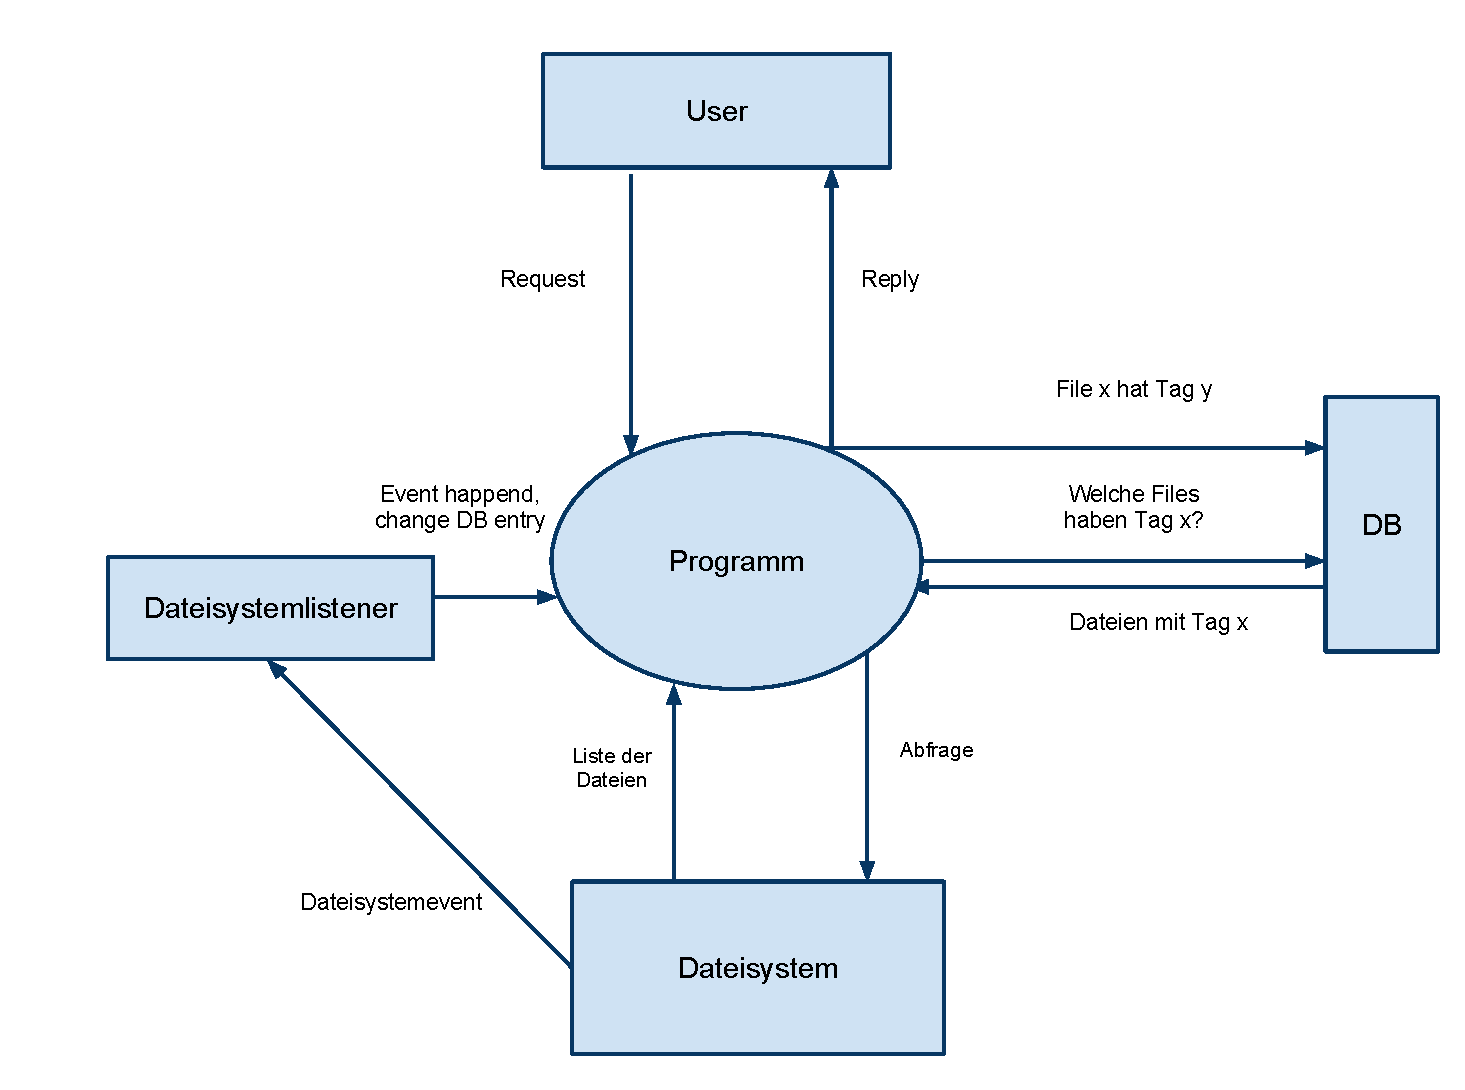
\includegraphics[width = \textwidth]{datenfluss.pdf}
    \caption{Datenflussdiagram}
    %\label{fig:hist}
  \end{figure}
\end{itemize}
\subsection{\"Ubersicht \"uber die erforderlichen Informationen / Daten}
\begin{itemize}
  \item vom Dateisystem
    \begin{itemize}
      \item Name der Datei
      \item Wo liegt die Datein (Verzeichnis)
      \item Andere Metadaten wie Zugriffsrechte, Datum der letzten Ver\"anderung, \ldots
    \end{itemize}
  \item von der Metadaten-Ablage
    \begin{itemize}
      \item Welche Tags wurden der Datei X zugeordnet
    \end{itemize}
  \item Dateisystem-Events
    \begin{itemize}
      \item Datei(en) wird/werden gel\"oscht
      \item Datei(en) wird/werden verschoben
      \item Datei wird ver\"andert
    \end{itemize}
\end{itemize}
\subsection{Anforderungen bez\"uglich Informationssicherheit und Datenschutz}
\begin{itemize}
  \item Informationssicherheit:  Verfügbarkeit, Vertraulichkeit, Integrität
    \begin{itemize}
      \item Die Verfügbarkeit des Programms hängt lediglich von der des Dateisystems ab und kann mit dieser gleichgesetzt werden.
      \item Das Vertrauen des Users wird gewonnen, indem nichts nach aussen (internet) geschickt wird.
      \item Die Integrität der Daten zu garantieren ist von daher eine Herausforderung, als dass das Programm mitbekommen muss, wenn Dateien verschoben werden und das registrieren muss. Ansonsten verweisen Metadaten ins Leere und Dateien verlieren die Ihnen zugeordneten 	Metadaten.\\
	Dieses Problem kann durch das Abhören von Dateisystem Events behoben werden.\\
	Umgehen liesse sich das Problem nur dann, wenn die Tags in den Filesystem-metadaten gespeichert würden.\\
    \end{itemize}
  \item Datenschutz
    \begin{itemize}
      \item Da das Programm lokal auf dem Computer läuft und nicht in die Zugriffsmechanismen des vorhandenen Systems eingreift geht die einzige Gefahr davon aus, dass der Speicherort der Tags für andere User frei zugänglich ist.\\
	Um das zu verhindern müssen die Tags entweder direkt in der jeweiligen Datei abgelegt werden oder, falls eine Datenbank zum Einsatz kommt muss diese in einem Verzeichnis abgelegt werden, auf das nur der jeweilige Benutzer Zugriff hat.
    \end{itemize}
\end{itemize}
\newpage
\section{L\"osungsvarianten}
\subsection{Zu verwendende Programmiersprache}
\subsubsection{L\"osungsvariante 1: Java}
\paragraph{Beschreibung der L\"osungsvariante}
Bei dieser L\"osung w\"urde Java als Programmiersprache f\"ur das Projekt verwendet. Java hat den Vorteil, dass der Interpreter eine sehr grosse Verbreitung geniesst und alle beteiligten Entwickler mit der Sprache vertraut sind.
\paragraph{Struktur (Grobe Architektur)}
Java hat sehr viele Module, die nicht nur die Entwicklung erleichtern, sondern auf den Zugriff auf verschiedene Formate, die zum Abspeichern der Daten verwendet werden k\"onnen.
\paragraph{Externe und interne Schnittstellen}
Wie bereits erw\"ahnt bietet Java viele Schnittstellen zu g\"angigen Datenbanken und Dateiformaten an.\\
Zudem hat Java verschiedene Frameworks die zur Erstellung des GUIs verwendet werden k\"onnen und sich zum Teil stark an den nativen Look des jeweiligen Systems anpassen.\\
Java’s Ausgabe in die Konsole hingegen ist eher langsam.\\
\paragraph{Abdeckung der Anforderungen}
\begin{itemize}
  \item {\bf Performance:} Java gilt heute als recht schnell.
  \item {\bf Flexibilit\"at:} Java gilt zur Zeit als die meist verwendete Programmiersprache \"uberhaupt, was den Vorteil mit sich bringt, dass sehr viele Programmierer in der Lage sind damit geschriebene Programme weiter zu entwickeln oder an zu passen.
  \item {\bf Sicherheit:} Dadurch dass Java code in der JVM ausgef\"uhrt wird, wird das ohnehin geringe Sicherheitsrisiko, dass durch den Einsatz der Software entsteht, noch weiter verringert.
  \item {\bf kompatibilit\"at:} Java ist f\"ur nahezu alle computer (egal ob Desktop oder handheld) verf\"ugbar, in verschiedenen Varianten, die teils selbst den hohen Offentheitsanspr\"uchen des Debian Projektes gen\"ugen. Die Verwendung vieler verschiedener Interpreter bringt aber auch Probleme. So sehen etwa Programme die f\"ur Sun/Oracle Java entwickelt wurden im Betrieb unter IcedTea etwas anders aus.
\end{itemize}
\paragraph{Realisierbarkeitsbetrachtung}
Die beteiligten Programmierer haben alle bereits Erfahrungen mit Java. Zudem findet man im Internet schnell Hilfe zu fast allen Bereichen der Programmiersprache.\\
Die Realisierbarkeit ist also durchaus gesichert wenn Java zum Einsatz kommt.
\subsubsection{L\"osungsvariante 2: Python}
\paragraph{Beschreibung der L\"osungsvariante}
Zur Implementierung des Programmes w\"urde hier Python verwendet. Die moderne Programmiersprache kommt heute immer \"ofters zum Einsatz und l\"auft auf allen g\"angigen Betriebssystemen.
\paragraph{Struktur (Grobe Architektur)}
Auch Python bietet Schnitstellen zu fast allen wichtigen Formaten und Datenbanken. Zudem bietet Python aber noch den Vorteil, dass es auch sehr viele low-level-Schnittstellen gibt, die auch sehr hardware (oder, hier von gr\"osserem Interesse, Dateisystem)nahe Operationen erlauben.
\paragraph{Externe und interne Schnittstellen}
Python braucht ebenfalls einen Interpreter. Dieser ist aber f\"ur alle g\"angigen Betriebssysteme verf\"ugbar. Zudem kann Python code auch in der weit verbreiteten Java Virtual Machine ausgef\"uhrt werden\cite{pyjava}.
\paragraph{Abdeckung der Anforderungen}
\begin{itemize}
  \item {\bf Performance} Python gilt als sehr performante Programmiersprache. Die Performance w\"urde f\"ur unseren Einsatzzweck vollauf gen\"ugen.
  \item {\bf Flexibilit\"at} Python hat ein ausgepr\"agtes Objekt Modell und ist gut Verst\"andlich. Zudem steigt die Zahl an Python Entwicklern seit einger Zeit sehr rasch. Auch eine in Python geschriebene Implementierung k\"onnte also sp\"ater gut von einem anderen Programmierer erweitert oder ge\"andert werden.
  \item {\bf Kompatibilit\"at} Der Python Interpreter hat eine deutlich weniger grosse Verbreitung als Java, ist aber auf Unix-artigen Systemen meist enthalten und kann unter Windows einfach installiert werden. Es l\"asst sich zudem spekulieren, dass Oracles aktueller Umgang mit Java und insbesondere mit der community der Verbreitung von Java starch schaden wird, wodurch dessen Verbreitung evtl. hinter die von Python zur\"uckfallen k\"onnte.
\end{itemize}
\paragraph{Realisierbarkeitsbetrachtung}
Der Einsatz von Python hat den Nachteil, dass die beteiligten Entwickler damit weniger vertraut sind als mit Java. Allerdings ist dadurch der Lerneffekt gr\"osser. Zudem bietet Python m\"achtige Module, die die Arbeit vereinfachen.\\
Python ist auch insbesondere f\"ur die Entwicklung von GUIs gut geignet. Unter Linux gibt es eine Vielzahl von Projekten, die lediglich ein Python GUI f\"ur Tools darstellen, die ansonsten nur f\"ur die Konsole verf\"ugbar sind.
\subsection{Zu verwendende Ablage f\"ur die Metadaten}
\subsubsection{L\"osungsvariante 1: SQLite}
\paragraph{Beschreibung der L\"osungsvariante}
ese Lösungsvariante sieht vor, dass die Daten in einer SQLite Datenbank abgelegt würden. SQLite scheint als Datenbank besonders gut geeignet, da alle Daten in lediglich einem File abgelegt werden. SQLite ist sehr schnell, unterstützt aber trotzdem alle standard SQL Befehle.\\
SQLite wird auch in populären Software Projekten wie Firefox und Adobe Air eingesetzt\cite{sqlite}.\\
\paragraph{Struktur (Grobe Architektur)}
  \begin{figure}[h!]
    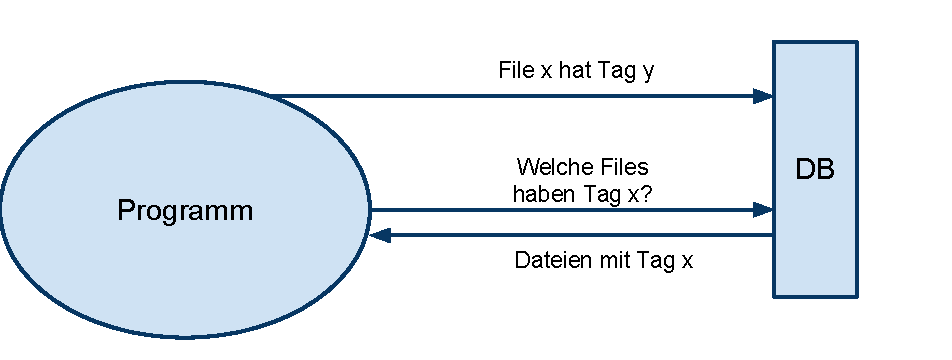
\includegraphics[width = \textwidth]{datenfluss_db.pdf}
    \caption{Datenflussdiagram beim Einsatz von SQLite}
  \end{figure}
\paragraph{Externe und interne Schnittstellen}
Dank der weiten Verbreitung von SQLite wird die leichtgewichtige Datenbank von fast allen Programmiersprachen unterstützt. Wie bei anderen Datenbanken auch, lassen sich darüber SQL Befehle absetzen, was das Speichern und Abfragen von Daten verhältnismässig sehr einfach macht.
\paragraph{Abdeckung der Anforderungen}
\begin{itemize}
  \item {\bf Performance} Performance: SQLite gilt als sehr schnelle Datenbank mit guten Caching. SQLite kann als die schnellste der hier vorgestellten Lösungen angesehen werden.
  \item {\bf Flexibilität} Flexibilität: Ein sauberes Datenbank-Layout lässt sich einfach erweitern, zudem wird SQLite von sehr vielen Programmiersprachen unterstützt, das macht diese Lösung sehr flexibel.
  \item {\bf Sicherheit} Sicherheit: Durch die Verwendung von SQLite würde kein weiteres Sicherheitsrisiko entstehen. Zwar besteht hier theoretisch das Risiko der SQL-injection. Da aber jeder User eine eigene Datenbank verwenden würde könnte auch niemand sonst code einschleusen. Umgekehrt würde das Einschleusen von Code wenig sinn machen, da ja kein anderer User die Datenbank jemals verwenden w\"urde.
  \item {\bf Kompatibilit\"at} Kompatibilität: SQLite ist für alle Betriebssyseme verfügbar.
  \item {\bf Datenkonsistenz} Datenkonsistenz: Da Datenbanken speziell für das Vermeiden von Datenkonsistenz entworfen wurden, kann diese Lösung hier besonders punkten. Natürlich müsste ein vernünftigen Datenbank-layout angelegt werden.
\end{itemize}
\paragraph{Realisierbarkeitsbetrachtung}
Die beteiligten Programmierer sind mit SQL vertraut. Zudem ist das Ansteuern von SQLite mit Python und Java sehr einfach. SQLite w\"are sicher am einfachsten um zu setzen.
\subsubsection{L\"osungsvariante 2: XML}
\paragraph{Beschreibung der L\"osungsvariante}
Diese Lösungsvariante sieht vor, dass die Metadaten in einem XML file abgelegt würden.\\
Dieses würde festhalten welche Datei (path und filename) welche Tags zugeordnet bekommen hat.
\paragraph{Struktur (Grobe Architektur)}
  \begin{figure}[h!]
    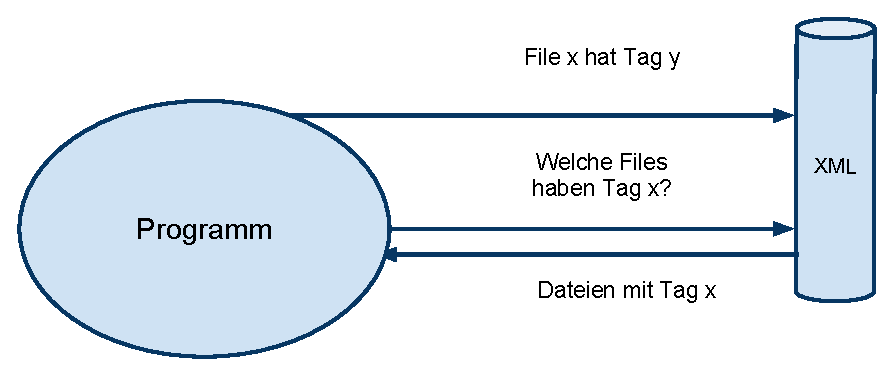
\includegraphics[width = \textwidth]{datenfluss_xml.pdf}
    \caption{Datenflussdiagram beim Einsatz von XML}
  \end{figure}
\paragraph{Externe und interne Schnittstellen}
So gut wie alle modernen Programmiersprachen haben Schnittstellen zu XML files die das Lesen und Schreiben der in XML Form abgelegten Daten einfach gestalten. XML gilt aber auch als schwerfällig und umständlich\cite{json}.
\paragraph{Abdeckung der Anforderungen}
\begin{itemize}
  \item {\bf Performance} Performance: Die Geschwindigkeit der XML Verarbeitung gilt als sehr gut und kann je nach Szenario durchaus mit der einer SQlite Datenbank mithalten.
  \item {\bf Flexibilität} Flexibilität: XML ist sehr flexibel und erlaubt auch das Erstellen eigener Definitionen. Zudem gibt es heute sehr viele Programmierer, die mit XML vertraut sind.
  XML brächte auch den Vorteil, dass die nurtext-Dateien auch ausserhalb des Programms problemlos gelesen und verarbeitet werden könnten.
  \item {\bf Sicherheit} Sicherheit: Bei der Verwendung von XML entstünden keine weiteren Sicherheitsprobleme.
  \item {\bf Kompatibilit\"at} Kompatibilität: Da die Daten in XML Files abgelegt wären, würde es keine Rolle spiele auf welchem System das Programm läuft. Die Kompatibilität und Portabilität wird also durch XML durchaus erhalten.
  \item {\bf Datenkonsistenz} Datenkonsistenz: Bei sauberem Ausarbeiten eines Layouts zum Abspeichern der Daten liesse sich mit XML die Datenkonsistenz problemlos erhalten.
\end{itemize}
\paragraph{Realisierbarkeitsbetrachtung}
Die beteiligten Programmierer sind mit dem Konzept von XML nicht weiter vertraut und müssten dieses zuerst erlernen. Besonders da XML zur Zeit stark von JSON bedrängt wird scheint das aber kaum sinnvoll.\\
Trotzdem wäre das Projekt bei Verwendung von XML sicher realisierbar.
\subsubsection{L\"osungsvariante 3: Metadaten des Dateisystems}
\paragraph{Beschreibung der L\"osungsvariante}
Eine Möglichkeit wäre es, die Daten zusammen mit der Datei auf das Dateisystem zu schreiben. Das bringt den Vorteil, dass die Informationen fest mit der Datei verbunden sind.
\paragraph{Struktur (Grobe Architektur)}
  \begin{figure}[h!]
    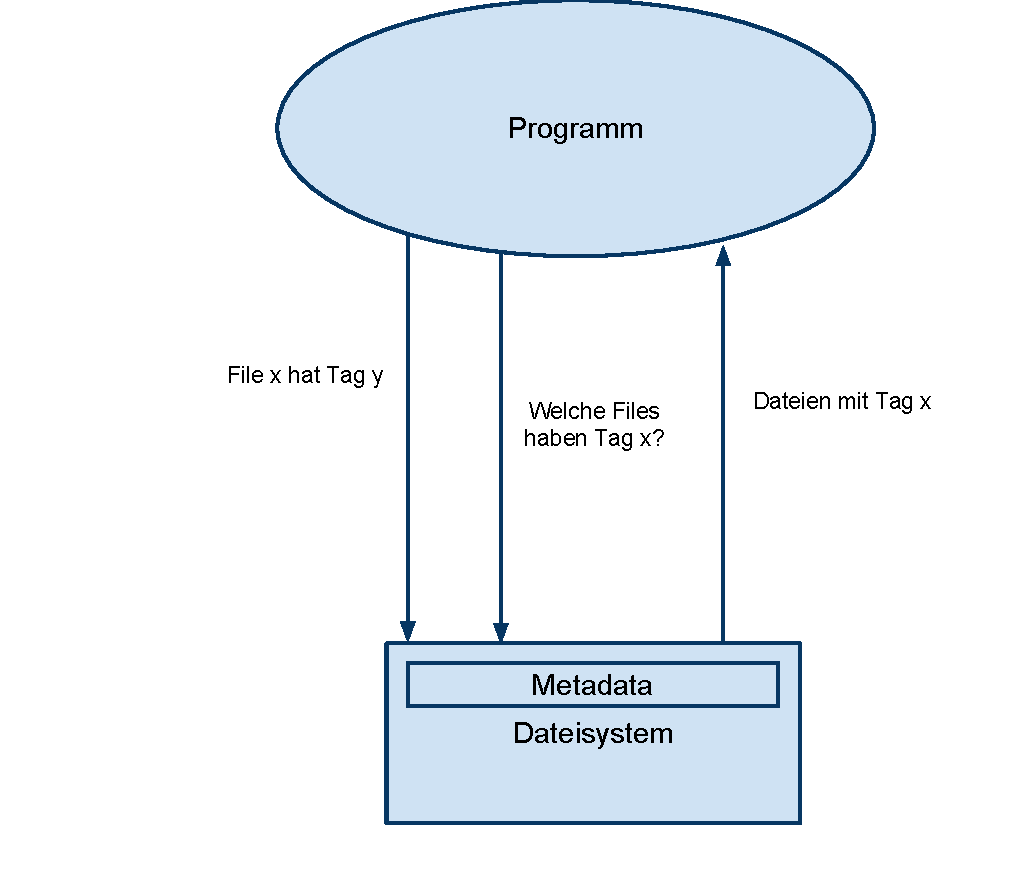
\includegraphics[width = \textwidth]{datenfluss_meta.pdf}
    \caption{Datenflussdiagram beim Speichern der Metadaten auf das Daeisystem}
  \end{figure}
\paragraph{Externe und interne Schnittstellen}
Die Schnittstellen die genutzt würden liegen beim Dateisystem. Das bringt das Problem mit, dass das Programm nicht auf allen Dateisystemen gleich arbeiten kann. Besonders in der Unix/Linux Welt wo es eine grosse Zahl verschiedener Dateisysteme gibt wäre das ein Problem.
\paragraph{Abdeckung der Anforderungen}
\begin{itemize}
  \item {\bf Performance} Performance: Wir haben einige Bedenken der Performance gegenüber. Da die Metadaten auf dem Dateisystem gespeichert würden, hätten wir keinen globalen Überblick darüber wo überall Dateien eines bestimmten Tags abgelegt sind und es müsste jedesmal eine Suche über das ganze Dateisystem laufen.\\
  Um das zu umgehen müsste eine zusätzliche Datenbank angelegt werden. Diese müsste aber mit den Daten des Dateisystems übereinstimmen und würde Redundanzen verursachen. Zudem würde das zusätzliche Betreiben einer Datenbank den Programmieraufwand erheblich steigern.
  \item {\bf Flexibilität} Flexibilität: Diese Lösung hätte den Nachteil, dass sie für verschiedene Dateisysteme angepasst werden müsste. 
  \item {\bf Sicherheit} Sicherheit: Falls diese Lösung verwendet würde würde evtl. auch eine Sicherheitslücke entstehen. Würden Daten auf einen externes Speichermedium kopiert, so würden die Metadaten mitkopiert. Werden aber Daten für eine Drittperson kopiert, so ist es nicht immer Wünschenswert wenn diese die Tags zu Gesicht bekommt.\\
  Man müsste also auch hier eine Lösung finden wie dieses Problem umgangen werden kann.
  \item {\bf Kompatibilit\"at} Kompatibilität: Grundsätzlich liesse sich diese Lösung wohl für die meisten Systeme realisieren. Sie müsste aber nicht nur für jedes System, sondern sogar für jedes Dateisystem angepasst werden.
  \item {\bf Datenkonsistenz} Datenkonsistenz: Die Lösung mit den Metadaten würde eine recht gute Datenkonsistenz schaffen, besonders da die Tags nicht verloren gingen, wenn eine Datei verschoben wird.\\
  Wie oben bereits erwähnt müsste aber wohl eine zusätzliche Datenbank angelegt werden, damit Suchbefehle auch in einem vernünftigen Zeitrahmen durchgeführt werden könnten. Diese zusätzliche Datenbank würde die Datenkonsistenz gefährden, vorallem da sie laufend mit den Daten des Dateisystems abgeglichen werden müsste.
\end{itemize}
\paragraph{Realisierbarkeitsbetrachtung}
Der Aufwand zur Realisierung dieser Variante währe weit grösser als bei den anderen Varianten. Nicht nur würde der Zugriff auf das Dateisystem, der sehr tief geht, implementiert werden, dieser müsste auch noch für verschiedene Systeme und Dateisysteme angepasst werden. Zudem müsste eine zusätzliche Datenbank angelegt werden, die laufend mit den Daten des Dateisystems abzugleichen wäre.\\
Diese Variante würde die Realisierung des Projektes stark gefährden!

\section{Entscheid über die Lösungsvarianten}
\subsection{Entscheidung zur zu verwendenden Programmiersprache}
\begin{tabularx}{\textwidth}{ |l|X|X|l|X|l| }
\hline
\bf Kriterium & \bf Wichtigkeit & \bf Java & \bf = & \bf Python & \bf = \\ \hline
Plattformunabhängig & 3 & 3 & 9 & 2 & 6\\ \hline
Kosten & 1 & 3 & 3 & 2 & 2 \\ \hline
Verbreitung des Interpreters & 2 & 3 & 6 & 1 & 2 \\ \hline
Geschwindigkeit & 1 & 2 & 2 & 3 & 3 \\ \hline
Einfachheit des Dateisystemzugriffs & 1 & 1 & 1 & 3 & 3 \\ \hline
Sofort ausf\"uhrbar & 1 & 1 & 1 & 3 & 3 \\ \hline
Lernwert & 2 & 1 & 2 & 3 & 6 \\ \hline
Offenheit des Systems & 2 & 2 & 4 & 3 & 6 \\ \hline
Gesammt & - & - & 28 \cellcolor{red!80!}& - & 31 \cellcolor{green!80!} \\ \hline
\end{tabularx}
\\
Anhand der oben abgebildeten Tabellen sind die jeweiligen Kriterien und die zugehörigen Bewertungen der Lösungsvarianten ersichtlich.\\
Zu trotzdem möchten wir hier noch einige Punkte hervorheben.\\
Bei den Programmiersprachen fiel die Wahl auf Python. Ausschlaggebend war hier, neben den genannten Kriterien, auch die Popularität der Sprache. Java ist zwar nach wie vor die meistverwendete Sprache, Python gewinnt aber sehr schnell an Beliebtheit und hat eine grosse und aktive User community.\\
Diese Beliebtheit und die aktuelle Nachfrage nach Python-Programmierern lässt vermuten, dass das Beherrschen der Scripting-Sprache für die spätere Berufssuche ein Vorteil sein könnte.
\subsection{Entscheidung zur zu verwendenden Ablage f\"ur die Metadaten}
\begin{tabularx}{\textwidth}{ |l|X|X|l|X|l|X|l|X| }
\hline
Kriterium & Wichtigkeit & SQLite & = & Metadaten & = & XML & = \\ \hline
Plattformunabhängigkeit & 3 & 3 & 9 & 1 & 3 & 3 & 9 \\ \hline
Datenbeständigkeit & 3 & 0 & 0 & 3 & 9 & 0 & 0 \\ \hline
APIs & 3 & 2 & 6 & 0 & 0 & 1 & 1 \\ \hline
Speicherbeanspruchung & 1 & 2 & 2 & 3 & 3 & 1 & 1 \\ \hline
Geschwindigkeit & 1 & 3 & 3 & 1 & 1 & 2 & 2 \\ \hline
Gesammt & - & - & 20 \cellcolor{green!80!}& - & 16 \cellcolor{red!80!}& - & 13 \cellcolor{red!80!} \\ \hline
\end{tabularx}
\\
Anhand der oben abgebildeten Tabellen sind die jeweiligen Kriterien und die zugehörigen Bewertungen der Lösungsvarianten ersichtlich.\\
Die Wahl der Speichermöglichkeit für die Tags fiel wesentlich einfacher als die Entscheidung für eine Programmiersprache. Zwar wäre das Verwenden der Filesystem-Metadaten sicherlich die technisch gesehen beste Lösung. Grösster Vorteil wäre, dass die Daten beim Kopieren der Datei in ein anderes Verzeichnis nicht verloren gingen.\\
Der Zugriff auf diese Metadaten ist aber recht kompliziert und erfordert tiefgehendes Verständnis des Filesystems. Auch ist nicht sichergestellt, dass diese Methode auf allen Dateisystemen eingesetzt werden kann.\\
SQLite bietet den Vorteil, dass gewöhnliche SQL-Befehle verwendet werden können. Die starke Auslegung unserer Ausbildung und unsere beruflichen Tätigkeiten haben dazu geführt, dass wir mit SQL gut vertraut sind.\\
Zudem gilt SQLite als sehr schnell.

%shylux
\section{Mittelbedarf}
\subsection{Sachmittel}
Sachmittel werden, neben den zur Verfügung stehenden Computern, keine benötigt.
\subsection{Personal}
Das Personal ist mit drei Programmierern vorgegeben.
\subsection{Ausbildung}
Mindestens zwei der Programmierer müssen sich Kenntnisse und Fähigkeiten im Umgang mit Python im Selbststudium aneignen.
Zudem muss der Umgang mit SQLite erlernt werden.
\subsection{Dienstleistungen}
Zur Zusammenarbeit und Recherche muss bei jedem Entwickler eine funktionierende Internetverbindung vorhanden sein.
Zudem werden zur Kommunikation und Zusammenarbeit die Officedienste und das Codeverwaltungstool von Google in Anspruch genommen. Um reine Textdateien zusammen zu bearbeiten benutzen wir Gobby.

\section{Planung und Organisation}
\subsection{Projektorganisation}
Das Team besteht aus zwei Programmierern und einem Projektmanager (PM).\\
Die Aufgabe des PMs wird im Verlaufe des Projektes weitergegeben.\\
Sollte der PM mit seiner Tätigkeit nicht ausgelastet sein, so wird er die Programmierer unterstützen.\\
Wahrscheinlich werden sich auch einige Spezialisierungen herausbilden. Es ist zum Beispiel denkbar, dass eine Person für das Datenbankdesign zuständig sein wird. Auch die Anpassung/Optimierung an die verschiedenen Betriebssysteme wird wohl jeweils einer einzelnen Person zufallen.
\subsection{Anwenderorganisation}
Die Anwender sind Einzelpersonen, die an einem lokalen Rechner arbeiten. Mehrere Personen könnten über freigegebene Ordner auf die Dateien zugreifen.
\subsection{Termine}
Die Termine sind von der Lehrkraft vorgegeben und im Terminplan eingetragen.
\subsection{Prioritäten}
Priorität hat die Schaffung einer GUI Version und die Dokumentation und die Überschaubarkeit des Codes.

\section{Wirtschaftlichkeit}
Vertrieb des Programms aussprechen wird, wird im Rahmen des Projektes keinerlei Umsatz generiert werden können. Ausserhalb des Projektes ist es natürlich möglich die von diesem Programmierer beigesteuerten Codeteile zu entfernen und das Programm zu vertreiben.\\
Ziel ist es, das Programm unter einer GPL oder BSD Lizenz zu veröffentlichen.\\
Es ist aber davon auszugehen, dass das Endprodukt bei der Verwendung einige Vorteile gegenüber herkömmlichen Dateimanagern bietet und dadurch Zeit eingespart werden kann. Das hängt vom Einsatzzweck ab und die dadurch entstehenden Kosteneinsprarungen könne nicht vorhergesagt werden.\\
Für uns bietet diese Projekt einen hohen Lernwert. Da wir selbst zu der Zielgruppe des Projekts gehören und es auch für uns optimieren können wir das Programm gut einsetzten.

\section{Konsequenzen}
\subsection{Auswirkungen (organisatorisch, personell, baulich, Vorschriften/Weisungen)}
Es stehen neue Wege zum Organisieren und Finden von Dateien zur Verfügung.\\
Das Organisieren von Projekten die sich über mehrere Ordner verteilen wird vereinfacht.\\
Die Beteiligten sammeln Erfahrungen mit den im Projekt eingesetzten Technologien.
\subsection{bei Nichtrealisierung}
Schlechte Note.
\subsection{bei verspäteter Realisierung (gegenüber Wunschtermin)}
Schlechte Note.
\subsection{auf Schnittstellen zu anderen Systemen}
Das Programm ist für den lokalen offline Einsatz vorgesehen. Onlinemodul falls wir genug Zeit haben.
\subsection{Qualitätsverbesserungen}
Einfacherer Umgang mit Dateien. Mehr Möglichkeiten zur Verwaltung von Dateien auf dem lokalen Betriebssystem.
\subsection{Risikobeurteilung}
Da das Team viel neues lernen muss und das Projekt recht viele einzelne Teile beinhaltet ist das Risiko, dass es nicht gänzlich fertiggestellt werden kann als beachtlich einzustufen.\\
Wenn das Programm keine Vorteile gegenüber anderen Dateiverwaltungstools beinhaltet, gerät das Programm in Vergessenheit.
\subsection{Ausweichmöglichkeiten}
Herkömmliche Dateimanager (explorer,bridge von adobe,ls,cp,rsync,mv,rm,find,locate).

\section{Antrag auf Freigabe der nächsten Projektphasen}
\subsection{bisherige Entscheide}
Als Programmiersprache haben wir Python bestätigt und als Datenbank haben wir SQLite gewählt.

\subsection{Formulierung des Antrags}
Wir haben uns eingehend mit den Zielen des Projekts befasst und eine realisierbare Lösung gewählt. Wir bitten sie deshalb den Antrag für die neue Phase zu genehmigen.


\end{document}